\documentclass[10pt]{article}
\usepackage{icmlko}

\icmlmeta{IP 파운데이션 월드모델}{264}{채우는 쪽을 적어 두기}{손으로 두 번 찾은 것을 가드로 옮겼다 --- 그리고 그 가드가 첫 판에 자기가 안 보는 값으로 판정했다}

\begin{document}

\twocolumn[
\icmlheader

\begin{abstract}
노트 262 · 263이 새는 축을 둘 찾았는데 둘 다 \textbf{손으로} 찾았다 --- 소스를
읽다가 우연히 봤다. 같은 틈이 또 있으면 또 우연에 기대야 한다. 그 틈의
정체는 분명하다: \texttt{provenance.WHEN} 은 축 \textbf{이름}에 뜻을 붙이는데
(\texttt{entry\_friction} $=$ ``기획서 태깅'') 손 축 다섯은 도메인마다 다른
필드로 채워진다. 그래서 \textbf{채우는 쪽 표}(\texttt{SOURCE}, 20쌍)를 적고
가드 열여덟 \textbf{쌓임}을 붙였다 --- 레코드에서 원본 필드를 꺼내 라벨을
안 보고 둘을 잰다: 연도와의 순위 상관, 유보 평균 대 학습 평균의 비.
\textbf{첫 실행에서 걸렸다}: 모바일 \texttt{media\_push}($\leftarrow$
\texttt{n\_shot}), 연도 $-$0.33, 비 4\%. 고치려고 재 보니 \textbf{판이
정확히 $+$0.0000} --- 노트 187의 제일 값싼 검사다. \texttt{n\_shot} 이 0 이면
축 빌더가 \emph{이미} 마스크 0 으로 내리고 있었고(86.4\%가 0 이다), 내
가드는 \textbf{모형이 안 보는 값으로 판정}하고 있었다. 관측된 행에서만 재도록
고치니 무늬가 사라진다. 고친 가드를 \textbf{막기 전 판}에 돌리니 손으로 찾은
둘을 그대로 문다 --- 웹툰 \texttt{entry\_friction}(연도 $-$0.44, 비 32\%)과
\texttt{goods\_scale}(연도 $-$0.49, 비 45\%). 지금 판에서는 원본 필드 13개를
검사하고 통과한다. \textbf{가드가 자기 검사에 한 번 걸린 것이 이 노트의
값이다} --- 가드도 축과 같은 규칙을 지켜야 한다.
\end{abstract}
]

\section{두 번 다 우연이었다}

노트 262는 \texttt{venue\_prominence} 의 정의를 확인하려고 소스를 열었다가
\texttt{entry\_friction} 이 \texttt{daily\_pass} 인 것을 봤다. 노트 263은
그 노트가 남긴 숙제를 따라 나머지를 훑다가 \texttt{goods\_scale} 이
\texttt{n\_episode} 인 것을 봤다. \textbf{둘 다 손으로 찾았다.}

틈의 정체는 분명하다.

\begin{center}\small
\begin{tabular}{ll}
\hline
\texttt{WHEN} 이 아는 것 & \texttt{entry\_friction}: PRE ``기획서 태깅'' \\
실제로 채우는 것 & 웹툰 \texttt{daily\_pass} · 애니 가격 · \\
 & 모바일 가격 · 만화 성인 여부 $\dots$ \\
\hline
\end{tabular}
\end{center}

한 이름에 뜻 하나를 붙였는데 아홉 도메인이 아홉 필드로 채운다. 여덟은 뜻이
맞고 하나는 안 맞았다.

\section{채우는 쪽 표와 가드 열여덟}

\texttt{provenance.SOURCE} 에 (도메인, 축) $\to$ 원본 필드를 20쌍 적었다.
가드 \textbf{쌓임}이 그 표를 읽어 레코드에서 필드를 꺼내 두 가지를 잰다.

\begin{center}\small
\begin{tabular}{ll}
\hline
검사 & 왜 \\
\hline
연도와의 순위 상관 & 쌓이는 양은 옛것일수록 크다 \\
유보 평균 / 학습 평균 & 쌓이는 양은 최근이 작다 \\
\hline
\end{tabular}
\end{center}

라벨을 안 본다 --- 노트 214의 한철, 노트 240의 겹말과 같은 부류다. 그리고
노트 263의 교훈대로 \textbf{유보 표본이 30건 미만이면 건너뛴다}(만화는 유보
여섯 건이라 ``학습 113 대 유보 44''가 여섯 건의 평균이었다).

\section{가드가 자기 검사에 걸렸다}

\begin{figure}[t]
\centering
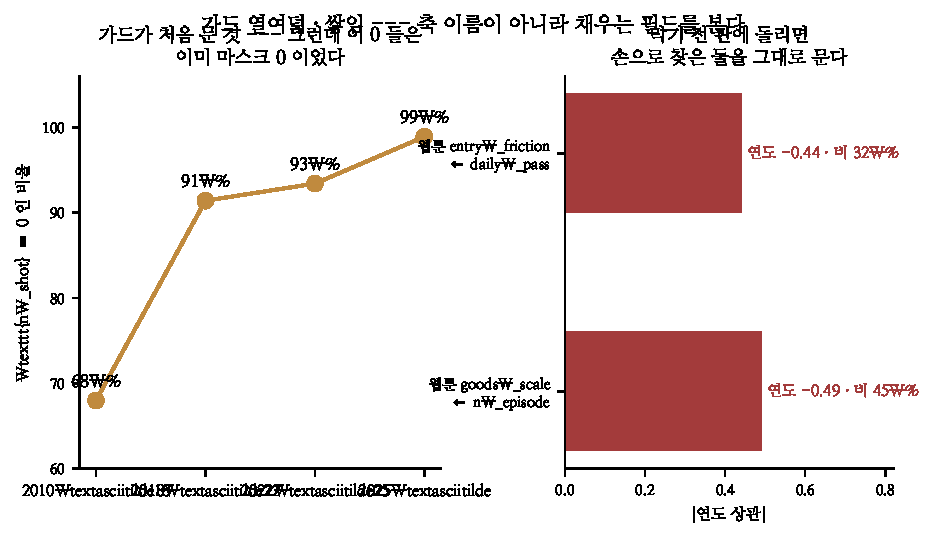
\includegraphics[width=\columnwidth]{figs/guard.pdf}
\caption{왼쪽 --- 가드가 처음 문 것. 오른쪽 --- 고친 가드를 막기 전 판에
돌린 결과.}
\end{figure}

첫 실행에서 하나 걸렸다.

\begin{quote}\small
모바일 \texttt{media\_push}(\texttt{n\_shot}) 연도 $-$0.33 비 4\% ---
예측 시점 뒤에 자란다
\end{quote}

비 4\% 는 웹툰(45\%)보다 훨씬 심하다. 그런데 스크린샷은 \emph{쌓이지 않는다}.
분포를 보니 0 인 비율이 최근일수록 오른다 --- 68\% $\to$ 91\% $\to$ 93\%
$\to$ 99\%. 쌓임이 아니라 \textbf{수집이 최근 것을 놓친 것}이다.

고치려고 두 가지를 쟀다 --- 0 을 결측으로 돌리기, 축을 통째로 막기.

\begin{center}\small
\begin{tabular}{lrr}
\hline
 & 판 & 짝 차 \\
\hline
지금 & 0.4842 & --- \\
0 을 결측으로 & 0.4842 & \textbf{$+$0.0000} \\
축 통째로 막음 & 0.4836 & $-$0.0006 \\
\hline
\end{tabular}
\end{center}

\textbf{정확히 $+$0.0000}. 노트 187의 제일 값싼 검사다 --- ``판이 넷째 자리까지
안 움직이면 효과가 없는 게 아니라 모형에 안 닿은 것''. 소스를 보니
\texttt{mobile\_axes.py} 가 \texttt{if ns:} 안에서만 값을 넣는다. \textbf{0 인
행은 이미 마스크 0 이었다.}

즉 내 가드는 \textbf{모형이 한 번도 안 보는 값 86.4\%를 섞어} 무늬를 만들고
있었다. 축이 지켜야 하는 규칙 --- 관측된 행에서만 읽는다 --- 을 가드가
안 지켰다.

\section{고치니 되짚어 문다}

관측 마스크를 씌우도록 고쳤다. 지금 판에서는 원본 필드 13개를 검사하고
\textbf{통과}한다. 그리고 \textbf{막기 전 판}(노트 262 이전)에 돌리면

\begin{quote}\small
웹툰 \texttt{entry\_friction}(\texttt{daily\_pass}) 연도 $-$0.44 비 32\% ·
웹툰 \texttt{goods\_scale}(\texttt{n\_episode}) 연도 $-$0.49 비 45\%
\end{quote}

\textbf{손으로 찾은 둘을 그대로 문다.} 우연에 기대던 것이 이제 자동이다.

\begin{center}\small
\begin{tabular}{lrl}
\hline
가드 & 개수 & \\
\hline
지금 판 & 9/9 & 쌓임 포함 전부 통과 \\
막기 전 판 & 8/9 & 쌓임 실패 (둘 지목) \\
\hline
\end{tabular}
\end{center}

\section{가드도 축과 같은 규칙을 지켜야 한다}

이 노트에서 실제로 배운 것은 표나 가드가 아니라 그 다음이다. 나는 노트
231에서 ``판정치가 죽은 것을 숨긴다''를 고쳤고, 노트 248에서 ``도메인별 수는
SE 와 함께''를 세웠고, 노트 261에서 ``실린 무게로 기여를 읽지 않는다''를
적었다. 전부 \emph{재는 쪽}의 규칙이다.

그런데 가드를 새로 쓸 때 그 규칙을 안 적용했다. \textbf{가드는 축을 검사하는
코드지 검사에서 면제된 코드가 아니다.} 이번엔 노트 187의 값싼 검사가
잡아 줬는데, 그 검사를 안 돌렸으면 모바일 축 하나를 근거 없이 막았을
것이다 --- 그리고 판이 안 움직이니 \emph{눈치도 못 챘을} 것이다.

\paragraph{남은 것}
\begin{center}\small
\begin{tabular}{ll}
\hline
갈래 & 왜 \\
\hline
\texttt{SOURCE} 채우기 & 20쌍 적었다. 손 축 $\times$ 도메인은 45쌍이다 \\
수집 편중 & \texttt{n\_shot} 0 이 최근 99\% --- 다시 긁으면 \\
23축 천장 & 두 번 막았으니 다시 재야 한다 \\
라벨 자체 & 노트 209의 누적 라벨. 축만 고쳤다 \\
\hline
\end{tabular}
\end{center}

\paragraph{규약} 새 가드를 붙이면 \textbf{그 가드가 이미 아는 사건을 되짚어
무는지} 먼저 확인한다. 이번엔 노트 262 · 263의 두 축이 시험지였고, 그것을
안 돌렸으면 가드가 틀린 채로 통과했을 것이다.

\end{document}
